% Presentatie Project 7 (tussentijds)
\documentclass{beamer}

\mode<presentation>

\usepackage[english]{babel}
\usepackage{listings}
%\usepackage{beamerthemesplit}

\lstset{ %
  language=bash,                % choose the language of the code
  basicstyle=\footnotesize,       % the size of the fonts that are used for the code
  numbers=left,                   % where to put the line-numbers
  numberstyle=\footnotesize,      % the size of the fonts that are used for the line-numbers
  numbersep=5pt,                  % how far the line-numbers are from the code
  showspaces=false,               % show spaces adding particular underscores
  showstringspaces=false,         % underline spaces within strings
  showtabs=false,                 % show tabs within strings adding particular underscores
  frame=lr,	                % adds left and right lines
  tabsize=2,	                % sets default tabsize to 2 spaces
  captionpos=b,                   % sets the caption-position to bottom
  breaklines=true,                % sets automatic line breaking
  breakatwhitespace=false,        % sets if automatic breaks should only happen at whitespace
%  escapeinside={\%*}{*)},         % if you want to add a comment within your code
  morekeywords={esac,fi,elseif,*,...}            % if you want to add more keywords to the set
}


%\usepackage{beamerthemesplit}
\usetheme{Berlin}
\useinnertheme{rounded}
\usecolortheme{rose}
\setbeamertemplate{navigation symbols}{} 

\title{phpBB\\Security and the feature}
\author{Paul Sohier}
\date{\today}

\begin{document}

\frame{
  \titlepage
} 

 \section{Introduction}
 \begin{frame}
   \frametitle{Introduction}
   \begin{itemize}
    \item<1-> Paul Sohier
    \item<1-> Official phpBB.com teammember
    \item<1-> \texttt{If you have any questions, please ask them at the end of the presentation}
   \end{itemize}
\end{frame}

\frame{
  \frametitle{Contents}
  \tableofcontents
}

\section{phpBB History}
\begin{frame}
  \frametitle{phpBB History}
  \begin{itemize}
    \item Founded in 2000
    \item Replacement for UBB
    \item Second version in 2002
    \item Third version in 2007
  \end{itemize}
\end{frame}

\section{phpBB Feature}
\begin{frame}
  \frametitle{phpBB Feature}
  \begin{itemize}
    \item Version 3.1 being developed
    \item Version 4 being planned
  \end{itemize}
\end{frame}

\begin{frame}
  \frametitle{Development times}
  \begin{itemize}
    \item Every is a volenteer
    \item Slow development
    \item Behind the market
  \end{itemize}
\end{frame}

\section{phpBB and Security}
\begin{frame}
  \frametitle{Security in phpBB2}
  \begin{itemize}
    \item Many issues caused by programming mistakes
    \item Large number of boards hacked
    \item Bad record for security
  \end{itemize}
\end{frame}

\begin{frame}
  \frametitle{phpBB 2.0.11, the never ever santy worm}
  \begin{itemize}
    \item First denied that it was a issue
    \item Fixed early december
    \item First boards hacked late december
  \end{itemize}
\end{frame}

\begin{frame}[fragile]
  \frametitle{phpBB 2.0.13, the equal mistake}
  \begin{itemize}
    \item Programming mistake, caused by php not being type strict
      \item \begin{lstlisting}
if (0 == false){echo ``yes'';}else{echo ``no'';}
      \end{lstlisting}
    \item Easy fix, large issues
    \item \begin{lstlisting}
if (0 === false) {echo ``yes'';}else{echo ``no'';}
      \end{lstlisting}
  \end{itemize}
\end{frame}

\begin{frame}
  \frametitle{phpBB3 security fixes}
  \begin{itemize}
    \item Require type strictness
    \item Require specific coding guidelines
    \item No serious issues since 2007
  \end{itemize}
\end{frame}

\begin{frame}
  \frametitle{Questions}
  Are there any questions?\\
    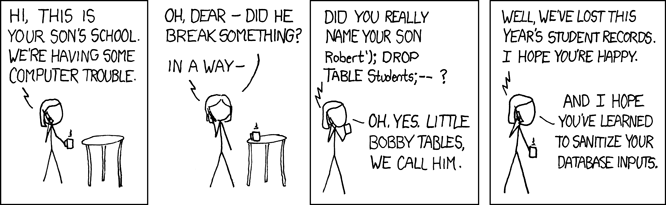
\includegraphics[scale=0.5]{exploits_of_a_mom.png}
\end{frame}

\end{document}
